% !TEX TS-program = tex
\documentclass[a4paper, 12pt]{article}

\usepackage{a4wide}
\usepackage[utf8]{inputenc}
\usepackage[russian]{babel}
\usepackage[pdftex]{graphicx}
\usepackage{amsmath}
\usepackage{amssymb}
\usepackage{amsfonts}
\usepackage{graphicx}
\usepackage{hyperref}
\usepackage{verbatim}
\usepackage{indentfirst}
\usepackage{listings}
% \usepackage{minted}
\setlength{\parindent}{1.25cm}

\newtheorem{myComment}{Замечание}
\newtheorem{myDef}{Определение}
\newtheorem{myProp}{Свойство}
\newtheorem{myTeor}{Теорема}
\newcommand{\dbtilde}[1]{\accentset{\approx}{#1}}
\DeclareMathOperator{\sign}{sign}

\begin{document}

\thispagestyle{empty}
\lstset{language=C++}

\begin{center}
\vspace{-3cm}

\includegraphics[width=0.5\textwidth]{msu.png}\\
{\scshape Московский государственный университет имени}\\
М. В. Ломоносова\\
Факультет вычислительной математики и кибернетики\\
Кафедра системного анализа

\vfill

% {\LARGE Отчёт по практикуму}

\vspace{1cm}

% {\Huge\bfseries <<Оптимальное управление>>}\\
{\LARGE Описание языка программирования Frigate}
\end{center}

\vspace{1cm}

\begin{flushright}
  \large
  \textit{Студент 415 группы}\\
  А.\,Н.~Ашабоков

  \vspace{5mm}

  \textit{Руководитель практикума}\\
  к.ф.-м.н., А.Н. Сальников 
\end{flushright}

\vfill

\begin{center}
Москва, 2019
\end{center}

\newpage
\setcounter{tocdepth}{1}
\tableofcontents

\newpage
\normalsize

\section{Общие сведения}

Система Frigate позволяет программисту представить свой алгоритм в виде графа состоящего из множества непересекающихся по вершинам подграфов. Каждый подграф является графом в смысле системы PARUS. Подграфы поочередно назначаются на исполнение. Этим управляет процесс координатор, адрес которого знают все вершины. Координатор содержит условные выражения, соответствующие каждому подграфу. На исполнение назначается тот подграф, чье выражение истинно. Данный механизм позволяет динамически перестраивать граф-программу во время выполнения, назначая на выполнение один из заранее подготовленных подграфов в каждый момент времени.
Ребра в графе бывают трех типов: внутренние (на уровне одного подграфа), внешние (на уровне графа соединяют подграфы), управляющие (на уровне графа направлены к процессу координатору). В целях уменьшения дублирования кода при создании большого количества подобных вершин или ребер был введен механизм шаблонов. Суть его в том, что программистом описывается шаблон вершины или ребра, содержащий все внутреннее устройство элемента, а при создании однотипных вершин или ребер, они используют описанный шаблон.
Вершины в графе Frigate могут иметь несколько точек входа и выхода ребер, чередующиеся с блоками обработки кода, таким образом достигается более сложная логика в работе кода вершины.
Программист описывает программу в синтаксисе языка Frigate, выделяя в программе последовательные участки обработки, соответствующие вершинам графа, и зависимости по данным - ребра. По данному представлению генерируется набор объектов в памяти, соответствующей иерархии классов. Затем из объектов-контейнеров генерируется набор функций с MPI- вставками, который компилируется на распределенной системе и связывается с подсистемой запуска.

\begin{center}
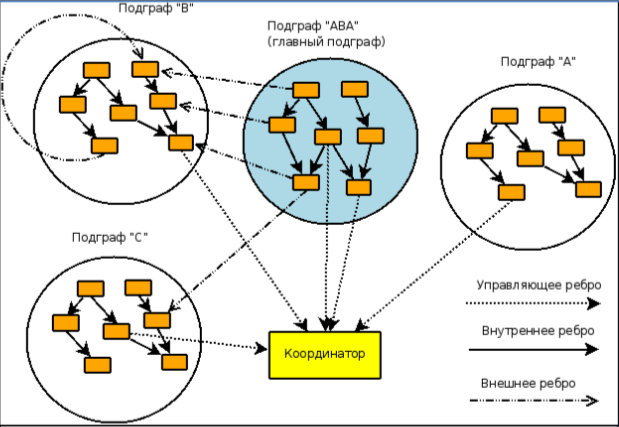
\includegraphics[width=0.7\textwidth]{pic_1.png}\\
Рис. 1: Общая схема графа программы на языке Frigate. \label{pic_3}
\end{center}

\section{Структура языка}

Программа на языке Frigate имеет следующую структуру:

\begin{lstlisting}
<graph>
	# Version of language
	version = 1.0
	
	<header>
		# the block that is copied to the beginning of the program
		@
			# block with C++ code
		@
	</header>
	
	<root>
		# block that runs at the 
		# very beginning of program execution
		root="file_with_root_code"
	</root>
	
	<tail>
		# block that runs at the end of program execution 
	</tail>
	
	# name of main subgraph
	main_subgraph="main"
	
	<subgraph>
		# subgraph description 
		name = "name_of_subgraph"
		condition = @ fulfillment condition @
		
		<vertex>
			# description of a vertex using a template
			name = "name_of_vertex"
			template = "name_of_vertex_template"
		</vertex>
		
		<vertex>
		# vertex description
			name = "name_of_vertex"
			
			<code>
				@
					# some code 
				@
			</code>
			
			<exchange>
				name = "name_of_exchange_block"
				send = "name_of_edge"
				...
				recv = "name_of_edge"
			</exchange>
			...
			<exchange>
				...
			</exchange>
			
			<code>
				...
			</code>
		</vertex>
		
		<internal_edge>
			# internal edge description
			name = "name_of_internal_edge"
			template = "name_of_template"
			send = ("name_of_sender_vertex", 
				"name_of_sender_exchange_block")
			recv = ("name_of_receiver_vertex", 
				"name_of_receiver_exchange_block")
		</internal_edge>
		
		...
		
		<control_edge>
			# control edge description 
			name = "name_of_control_edge"
			template = "name_of_control_edge"
			send = ("name_of_sender_vertex", 
				"name_of_sender_exchange_block")
		</control_edge>
	</subgraph>	

	...	
	
	<subgraph>
		...
	</subgraph>
	
	<external_edge>
		# external edge description 
		name = "name_of_external_edge"
		template = "name_of_edge_template"
		send = ("name_of_sender_subgraph", 
			"name_of_sender_vertex", 
			"name_of_sender_exchange_block")
		recv = ("name_of_receiver_subgraph", 
			"name_of_receiver_vertex", 
			"name_of_receiver_exchange_block")
	</external_edge>
	
	...
	
	<edge_template>
		# edge template description 
		name = "name_of_edge_template"
		
		<send>
			# msg description
			<fragment>
				# data description
				variable = @   @
				type = @   @
				left = @   @
				right = @   @
			</fragment>
			...
			<fragment>
				...
			</fragment>
		</send>
		
		<recv>
			...
		</recv>
	</edge_template>
	...
	
	<vertex_template>
		# vertex template description 
		name = "name_of_vertex_template"
		
		<code>
			io_volume = @ ... @
			file = "name_of_file_with_code"
		</code>
		...
		<code>
			io_volume = @ ... @
			code_volume = @ ... @
			@
				# code block
			@
		</code>
		...
		<exchange>
			name = "name_of_exchange_block"
			send = "name_of_edge"
			..
			recv = "name_of_edge"
		</exchange>
	</vertex_template>
</graph>
\end{lstlisting}
Перед началом разбора структуры языка введем следующие договоренности:
\begin{itemize}
	\item Поле \lstinline$name$ внутри любого из объектов содержит имя данного объекта
	\item Блок вида $@$...$@$ содержит некоторый исполняемый код на языке C++. Пример:
	\begin{lstlisting}
		@
			int a = 1;
			int b = 2;
			int c = a + b;
		@
	\end{lstlisting}
\end{itemize}
Везде далее объяснения значений этих полей будут опущены.

Программа на языке Frigate описывается в виде графа, внутри блока <graph> содержится описание всех подграфов \lstinline$<subgraph>$, шаблонов вершин \lstinline$<vertex_template>$, шаблонов ребер \lstinline$<edge_template>$ и внешних ребер \lstinline$<external_edge>$, соединяющих вершины различных подграфов, а также содержит блоки \lstinline$<header>$, \lstinline$<root>$ и \lstinline$<tail>$. 
\begin{itemize}
\item Блок \lstinline$<header>$  содержит в себе код на языке \lstinline$C++$, который при компиляции MPI программы будет прямиком скопирован в его начало. 
\item Блок \lstinline$<root>$ содержит код C++, который выполняется MPI программой перед началом каких-либо действий. Его имеет смысл использовать для проведения подготовительных работ перед началом работы основного вычислительного алгоритма, например для инициализации каких-либо глобальных переменных и выделения памяти. 
\item Блок \lstinline$<tail>$ содержит код \lstinline$C++$, который выполняется каждой вершиной по завершению основных вычислений. Данный блок можно использовать, например, для очищения выделенной памяти. 
\item Поле \lstinline$main_subgraph$ содержит имя подграфа, который далее будет считаться главным.
\end{itemize}
Рассмотрим теперь структуру подграфа \lstinline$<subgraph>$. Подграф содержит описание все своих вершин \lstinline$<vertex>$, внутренних ребер \lstinline$<internal_edge>$ и управляющих ребер \lstinline$<control_edge>$. Сразу отметим, что эти блоки могут идти в произвольном порядке.
\begin{itemize}
\item Поле \lstinline$condition$ содержит условие выполнения данного подграфа на языке C++.
\item Блок \lstinline$<vertex>$ содержит описание вершины данного подграфа. Вершины могут быть описаны либо явно внутри подграфа, либо при помощи шаблона вершины (см. далее), путем задания в поле \lstinline$template$ имя используемого шаблона. Очевидно, что использование шаблонов вершины имеет смысл в том случае, когда требуется создать большое количество однотипных вершин, реализующих один и тот же алгоритм. Явное описание вершины совпадает с описанием шаблона вершины и приведено далее по тексту. 
\item Блок \lstinline$<internal_edge>$ содержит описание внутренних ребер подграфа. Очевидно, эти ребра могут быть использованы только для связи вершин внутри одного подграфа, для коммуникации с вершинами других подграфов необходимо использовать внешние ребра \lstinline$<external_edge>$. Внутреннее ребро содержит следующие поля:
	\begin{itemize}
		\item Поле \lstinline$template$ содержит название шаблона ребра, используемого данным ребром.
		\item Поле \lstinline$send$ содержит адрес отправителя в формате: $("$название вершины отправителя$"$, $"$название exchange блока отправителя$")$.
		\item Поле \lstinline$recv$ аналогично содержит адрес отправителя: $("$название вершины получателя$"$, $"$название exchange блока получателя$")$.
	\end{itemize}
\item Блок \lstinline$<control_edge>$ содержит описание ребра, соединяющего вершину с координатором. Очевидно, что в \lstinline$<control_edge>$ нет необходимости описания адреса получателя. т.к. это всегда процесс-координатор. Структура ребра:
	\begin{itemize}
		\item \lstinline$template$ --- название используемого шаблона вершины.
		\item \lstinline$send$ --- адрес отправителя, в том же формате, что и для \lstinline$<internal_edge>$.
	\end{itemize}
\end{itemize}
Рассмотрим структуру блока \lstinline$<external_edge>$. Данный блок содержит описание внешней вершины, соединяющей вершины различных подграфов. Фактически структура внешнего ребра \lstinline$<external_edge>$ отличается от структуры внутреннего ребра \lstinline$<internal_edge>$ только набором параметром, задающих адрес отправителя и получателя. Это связано с тем, что при передаче данныз внутри определенного прдграфа, знание имени подграфа не является необходимым, что, очевидно, неверно для внешних ребер,
\begin{itemize}
	\item Поле \lstinline$template$ содержит название используемого шаблона ребра.
	\item Поле \lstinline$send$ содержит адрес отправителя в формате: $("$название подграфа отправителя$"$, $"$название вершины отправителя$"$, $"$название exchange блока отправителя$")$.
	\item Поле \lstinline$recv$ аналогично содержит адрес отправителя: $("$название подграфа получателя$"$, $"$название вершины получателя$"$, $"$название exchange блока получателя$")$.
\end{itemize}
Дополнительно отметим, что в поле с адресом вместо имени вершины можно указать имя шаблона вершины, это будет значить, что для каждой вершины, использующей указанный шаблон, компилятор автоматически создаст дубликаты этого ребра. Это необходимо для того, чтобы обеспечить гармоничную работу ребер с вершинами, созданными с использованием шаблонов вершин. Приведем пример:
\begin{lstlisting}
...

<vertex>
	name = "first_vertex"
	template = "first_template"
</vertex>

<vertex>
	name = "second_vertex"
	template = "first_template"
</vertex>

<vertex>
	name = "third_vertex"
	template = "second_template"
</vertex>

<internal_edge>
	name = "first_internal_edge"
	template = "first_edge_template"
	send = ("first_template", "first_exchange")
	recv = ("third_vertex", "first_exchange")
</internal_edge>

<internal_edge>
	name = "second_internal_edge"
	template = "first_edge_template"
	send = ("first_vertex", "first_exchange")
	recv = ("second_vertex", "first_exchange")
</internal_edge>

...
\end{lstlisting}
В данном примере ребро \lstinline$"first_internal_edge"$ соединяет вершины \lstinline$"first_vertex"$ и \lstinline$"second_vertex"$ с вершиной \lstinline$"third_vertex"$, т.к. описание ребра содержит название шаблона вершины, а ребро \lstinline$"second_internal_edge"$ соединяет вершины \lstinline$"first_vertex"$ и \lstinline$"second_vertex"$, т.к. описание ребра содержит явные названия вершин.

Рассмотрим структуру блока \lstinline$<edge_template>$. Этот блок содержит описание блоков памяти, содержащих данные для отправки по указанному ребру, и блоки памяти, в которые получаемые данные должны быть сохранены.
\begin{itemize}
	\item Блок \lstinline$<send>$ содержит в себе перечисление некоторого числа блоков \lstinline$<fragment>$ ---  фрагментов памяти, подлежащих отправке по данному ребру. Блок \lstinline$<fragment>$ имеет структуру:
		\begin{itemize}
			\item Поле \lstinline$variable$ --- название переменной.
			\item Поле \lstinline$type$ --- тип передаваемых данных.
			\item Поле \lstinline$left$ ---  указатель на левую границу массива с данными в памяти.
			\item Поле \lstinline$right$ ---  указатель на правую границу массива с данными в памяти.
		\end{itemize}
	 \item Блок \lstinline$recv$ содержит перечисление блоков \lstinline$<fragment>$ --- фрагментов памяти, в которые произойдет сохранение полученных по данному ребру данных. Структура блока \lstinline$<fragment>$ описана выше.
\end{itemize}
Рассмотрим структуру блока \lstinline$<vertex_template>$. Структура данного блока совпадает со структурой блока \lstinline$<vertex>$ в том случае, когда вершина задается не через шаблон вершины, а явно внутри блока \lstinline$<vertex>$. Блок \lstinline$<vertex_template>$ состоит из произвольного количества блоков \lstinline$<code>$ и \lstinline$<exchange>$ в произвольном порядке.
\begin{itemize}
	\item Блок \lstinline$<code>$ содержит исполняемый код на языке C++. Его можно задать вписав код в специальный блок вида $@$...$@$, либо подключив файл с кодом на C++, указав название файла в поле \lstinline$file$.
	\item Блок \lstinline$<exchange>$ отвечает за обмен данными между вершинами. Управление обменом осуществляется при помощи полей \lstinline$send$ и \lstinline$recv$:
	\begin{itemize}
		\item Поле \lstinline$send$ содержит название ребра, по которому будет осуществляться отправка данных.
		\item Поле \lstinline$recv$ содержит название ребра, по которому будет осуществляться получение данных.
	\end{itemize}
	Дополнительно отметим, что блок \lstinline$<exchange>$ может состоять из произвольного количества полей \lstinline$send$ и \lstinline$recv$, перечисленных в произвольном порядке. Это значит, что один \lstinline$<exchange>$ блок может осуществлять произвольное число операций передачи и получения данных в произвольном порядке. Также стоит отметить, что возможно чередование блоков \lstinline$<code>$ и \lstinline$<exchange>$. Это значит, что вершина по мере выполнения может отправлять промежуточные данные и получать их от других вершин.
\end{itemize}

%\section{Соглашения об уникальности имен}
%
%Очевидно, что представление программы в виде графа может привести к тому, что полученный граф будет иметь довольно сложную структуру, что естественным путем приводит к необходимости введения пространств видимости имен.
%
%\begin{itemize}
%	\item Имена подграфов \lstinline$<subgraph>$ не могут совпадать
%	\item Имена вершин \lstinline$<vertex>$ внутри одного подграфа не могут совпадать
%	
%\end{itemize}

\section{Пример программы}

\begin{lstlisting}


# hello
# hello
<graph>	
	#
	# Version of Graph format
	#
	version = 1.0
	
	<header>
		@
		       msdl;jsfgjdfglkjfsl;gkhj
		       g,fsg,hjdf;glkjf;lgjflgkhj
		       g;lhdfg;lhjkdf;ljfsd;khlj
		      \@
		      \@
		       ffghdfgfghfg
		       fghdfghfgh
		@
	</header>
	
	<root>	
	    root="ddd"
	</root>
	
	<tail>
		@
		Now it is code
		fghdfghdfghf
		fghdfghf
		@
	</tail>
	
	
	# main_subgraph="hello \"world\""
	main_subgraph="world"
	
	<subgraph>
		name # hello
		 = # dddd
		"world"
		#
		# beee
		#
		
		condition = @ 1 @
		
		<vertex>
			name="abba"
			template = "generic"
		</vertex>
		
		<vertex>
			name="bbb"
			
			<code>
				file="hello"
			</code>
			
			<code>
				@
				 if(a==0)
				 {
				  a=10;
				 }
				@
			</code>
			
			<code>
				io_volume  = @ 0       @
				code_volume= @ abc*bca @
				@
				 if(a==0)
				 {
				  a=10;
				 }
				@
			</code>
			
			<exchange>
			    name="first"
			    send="my first internal edge"
			    send="my first control edge"
			    recv="my second internal edge"
			    recv="my first external edge"
			</exchange>

			<exchange>
			    name="second"
			    send="my fifth internal edge"
			    send="my third control edge"
			    recv="my fourth internal edge"
			    recv="my third external edge"
			</exchange>
					
		</vertex>
		
		<internal_edge>
		    name="my first internal edge"
		    template="first"
		    send=("bbb","first")
		    recv=("abba","first")
		</internal_edge>

		<internal_edge>
		    name="my second internal edge"
		    template="first"
		    send=("abba","first")
		    recv=("bbb","first")
		</internal_edge>

		<internal_edge>
		    name="my third internal edge"
		    template="first"
		    send=("bbb","first")
		    recv=("abba","first")
		</internal_edge>

		<internal_edge>
		    name="my fifth internal edge"
		    template="first"
		    send=("bbb","second")
		    recv=("abba","first")
		</internal_edge>

		<internal_edge>
			name = "my fourth internal edge"
			template = "first"
			send= ("abba", "first")
			recv = ("bbb", "second")
		</internal_edge>
		
		<control_edge>
		    name="my first control edge"
		    template="first"
		    send=("bbb","first")
		</control_edge>

		<control_edge>
		    name="my third control edge"
		    template="first"
		    send=("bbb","second")
		</control_edge>


		<control_edge>
			name = "my second control edge"
			template = "first"
			send = ( "abba" , "first" )
		</control_edge>

	</subgraph>
	
	<edge_template>
	    name="first"
		 <send>   
		    <fragment>
		        variable = @a["offset"]@
		        type     = @ my_mpi_type["offset"] @
		        left     = @ (i-1)*global_size/num_vertices @
		        right    = @ i*global_size/num_vertices     @
		    </fragment>
		
		    <fragment>
		        variable = @a["offset"]@
		        type     = @ my_mpi_type["offset"] @
		        left     = @ (i-1)*global_size/num_vertices @
		        right    = @ i*global_size/num_vertices     @
		    </fragment>
		
		 </send>
	
		 <recv>
		    <fragment>
		        variable = @a["offset"]@
		        type     = @ my_mpi_type["offset"] @
		        left     = @ (i-1)*global_size/num_vertices @
		        right    = @ i*global_size/num_vertices     @
		    </fragment>
		 </recv>
	</edge_template>
	
	<external_edge>
	    name="my first external edge"
	    template="first"
	    send=("world","abba",  "first")
	    recv=("world","bbb" , "first")
	</external_edge>

	<external_edge>
	    name="my third external edge"
	    template="first"
	    send=("world","abba",  "first")
	    recv=("world","bbb" , "second")
	</external_edge>


	<external_edge>
	    name="my second external edge"
	    template="first"
	    send=("world","bbb",  "first")
	    recv=("world","abba" , "first")
	</external_edge>

	
	<vertex_template>
	    name="generic"
	    
	    <code>
	        io_volume = @ a+bbbb @
	        file="hello"
	    </code>
	
	    <code>
	        @
             if(a==0)
             {
               a=10;
             }
	        @
	    </code>
	
	    <code>
	        io_volume  = @ 0       @
	        code_volume= @ abc*bca @
	        @
	             if(a==0)
	             {
	                a=10;
	             }
	        @
	    </code>
	
	    <exchange>
	        name="first"
	        
	        send="my second control edge"
	        send="my second internal edge"
	        
	        recv="my second external edge"
	        recv="my third internal edge"
	    </exchange>

		
	</vertex_template>

</graph># gfghfghfg
# hello
# ehlo
\end{lstlisting}


\end{document}